\documentclass[conference]{IEEEtran}
\usepackage{amsmath,amssymb,booktabs,graphicx,xcolor}
\usepackage[hidelinks]{hyperref}
\usepackage{url}
\usepackage{balance}
\usepackage{iftex}
\ifXeTeX
\usepackage{fontspec}
\setmainfont{texgyretermes-regular.otf}[BoldFont=texgyretermes-bold.otf,ItalicFont=texgyretermes-italic.otf,BoldItalicFont=texgyretermes-bolditalic.otf]
\setsansfont{texgyreheros-regular.otf}[BoldFont=texgyreheros-bold.otf,ItalicFont=texgyreheros-italic.otf]
\setmonofont{texgyrecursor-regular.otf}[BoldFont=texgyrecursor-bold.otf]
\fi
\definecolor{forest}{RGB}{32,75,64}
\title{Maintaining Source-Linked Evidence Views for Agent Memory}
\author{}
\begin{document}
\maketitle
\begin{abstract}
An agent must fit jointly useful evidence into context and revise it when execution sources change. Our SQLite consoles maintain and audit budgeted evidence packets for tool traces and code edits. On 2,000 ISETrace queries, learned packing recovered all annotated spans in 83.07\% of cases versus 81.19\% for first-fit on the same graph ranking. Across 40,000 graph-reader states, conservative variable elimination reproduced every original floating-point packet and reduced warm selection time by $2.13\times$. On 1,071 observed code edits, local alignment preserved 323 complete packets versus 302 with range invalidation. Visitors advance a trace, revise a source and verify the exact output.

\end{abstract}

\section{Why maintain the evidence packet?}

A memory query may require an invocation and a later result in the same context. If a source disappears, must we rerun retrieval? In the demo, excluding one call replaces unit 11 with unit 19 at identical cost and coverage. Another exclusion needs no optimization. Even removal of an unselected candidate can affect the answer.

Wang et al.\ use provenance to retrieve supporting spans \cite{wang}. Bala and Feng et al.\ study bounded context and coding-agent states \cite{bala,feng}. MemTrace validates trace anchors at restore time \cite{memtrace}. PACMI propagates validity changes \cite{pacmi}. Snapshot reads \cite{readboundaries} and executable workflows \cite{changes} address changes in stored facts. We ask when an optimal packet survives a revision within a coherent snapshot.

Yi et al.\ retain extra ranked tuples to reduce refills in materialized top-$k$ views \cite{topk}. Here a cumulative-cost prefix constrains a second optimization. TAPE demonstrates temporal graph memory for personal agents \cite{tape}. Our visitor inspects which provenance dependencies suffice to reuse this two-stage selection. Runtime work on evolving coding-agent state tracks which observations remain current \cite{execledger}. We additionally track when a valid observation can change the bounded answer.

\begin{figure}[t]
\centering
\setlength{\fboxsep}{4pt}
\begin{tabular}{@{}c@{}}
\fcolorbox{forest}{white}{\parbox{.88\columnwidth}{\centering \textbf{Public execution trace}\\Events, argument/output fields and character offsets}}\\
$\downarrow$\\
\fcolorbox{forest}{white}{\parbox{.88\columnwidth}{\centering \textbf{Read-only SQLite projection}\\Unit, source span, directed relation, cost, rank, utility}}\\
$\downarrow$\\
\fcolorbox{forest}{white}{\parbox{.88\columnwidth}{\centering \textbf{Materialized view and source dependencies}\\Protected prefix, packed suffix and prefix boundary}}\\
$\downarrow$\\
\fcolorbox{forest}{white}{\parbox{.88\columnwidth}{\centering \textbf{Live visitor controls}\\Exclude a source, inspect a unit, compare maintenance plans}}\\
\end{tabular}
\caption{Serving architecture. A separate evaluator receives the resulting unit IDs and compares their source intervals with a private annotation table on demand. The selection path has no access to that table or to the bodies of tool calls.}
\label{fig:system}
\end{figure}

\section{Selection and source dependencies}

\subsection{Materializing a view}
Candidate $i$ has cost $c_i\geq0$, utility $u_i$ and source intervals (event, field, half-open character offsets). Costs add across selected candidates. Evaluation merges overlapping intervals in source coordinates.

Let $B$ be the token budget and $T\leq B$ the prefix threshold. Protect the longest consecutive prefix $H$ costing at most $T$; the first candidate outside $H$ is its boundary. The first-fit comparator scans the entire ranking, admitting any candidate that still fits.

A gradient-boosted tree estimates candidate membership in the annotated evidence from graph and dense rank, type, cost, graph score and gap to the leader, and pool size. We fit it on 3,894 training queries weighted equally and transform its log-odds into positive utility with softplus. Joint sufficiency is measured separately on held-out queries.

Write $C=B-\sum_{i\in H} c_i$. On the remaining candidates the selector maximizes $\sum_i u_i x_i$ subject to $\sum_i c_i x_i\leq C$ and $x_i\in\{0,1\}$. A standard exact dynamic program updates the value at each integer capacity. Ties keep the existing solution. We return selected IDs in their original rank order. Threshold selection on 580 validation queries gave $T=1,024$ at $B=2,048$. Other thresholds trade a larger fixed prefix against additional freedom for the optimizer. The contribution here is a materialized packet with auditable source dependencies and maintenance rules.

\subsection{When can an exclusion change a packet?}
Let $P$ denote the stored packet and $D$ the set of candidate IDs removed by one or more source exclusions. Surviving candidates retain their order, costs and utilities. Fix the budget, threshold, and one total order on tied complete packets, including when a suffix item becomes mandatory. Let $H'$ be the protected prefix recomputed on the remaining candidates.

\textbf{Reuse criterion.} The ordered packet is unchanged exactly when
\[
           D\cap P=\varnothing \quad\text{and}\quad H'\subseteq P.
\]
If a selected unit is removed, its ID cannot survive. If the new prefix contains a previously unselected unit, the new packet must contain that unit. For sufficiency, the first condition implies that all members of $H$ survive. Deletions can extend this prefix, so $H\subseteq H'$. By the second condition the old optimum contains every newly mandatory unit and remains feasible. Every packet feasible under the new requirement was already feasible before deletion. On these nested feasible families a previous optimum remains optimal, and the stable tie rule preserves its identity. Rank order of the surviving units is unchanged, giving equality of the ordered packets. With exact comparisons, strict-update dynamic programming preserves this order by preferring absence at the last differing rank. A signed 64-bit implementation with fixed-point Q32 utilities reproduced all 10,000 original packets and all 108,204 deletion outcomes. The maximum tested utility sum was 13,789,213,370. Arbitrary floating-point summation orders do not inherit this guarantee.

A faster sufficient certificate indexes all sources of selected units and of the boundary. If an exclusion touches none of them, the old prefix survives and the suffix loses only unselected candidates. An index hit triggers recomputation, including some cases where the exact criterion would allow reuse.

For example, let $(B,T)=(8,4)$, costs $(3,3,1,5)$ and utilities $(1,1,3,10)$. Prefix $(0)$ and suffix $(3)$ fit. Removing unselected unit 1 forces prefix $(0,2)$ and leaves 4 tokens: unit 3 no longer fits.

\section{Implementation and visitor interaction}

SQLite stores query-local units, costs, utilities, source spans and typed edges. A parameterized anti-join excludes units attached to a removed source.

The trace projection contains 5,009 units and 10,789 typed edges for 40 hash-sampled queries from separate trajectories. ISETrace contains real tool executions for synthetic OS-agent tasks \cite{ise,wang}; we simulate source exclusions. A streaming projection replays arrivals and support updates from SQLite. A separate projection uses actual edits from Handoff Debt \cite{handoff}. Anonymized serving tuples and independent audit witnesses ship with the local consoles.

\begin{figure*}[t]
\centering
\begin{minipage}[t]{.48\textwidth}\vspace{0pt}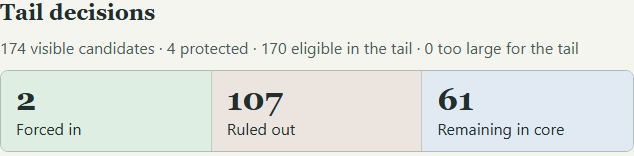
\includegraphics[width=\linewidth]{core.png}\end{minipage}\hfill
\begin{minipage}[t]{.48\textwidth}\vspace{0pt}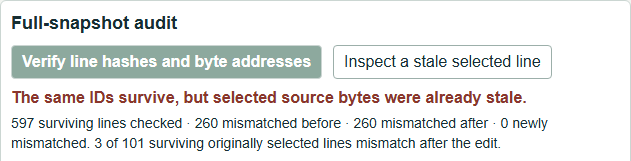
\includegraphics[width=\linewidth]{edit.png}\end{minipage}
\caption{Two running consoles. Left, bounds on learned utility force 2 candidates and exclude 107 in a recorded graph state. Right, a coding-agent edit retains the selected block IDs, yet the snapshot check detects incorrect line addresses in the original display. The audit operates separately from selection.}
\label{fig:ui}
\end{figure*}

\subsection{Visitor scenarios}
\textit{Change source evidence.} Exclude an unused q02 source, then a selected one: unit 19 replaces unit 11. The independent audit finds all 60 annotated characters. Stepping across one weight breakpoint changes nine units to thirteen. In \emph{Two sources}, each q03 shift alone preserves the packet; applying both changes it. In \emph{Observed updates}, replay q25's six producer changes. Each alone preserves 19 fragments; the transaction selects 15 under the count policy.

\textit{Change the budget or boundary.} Reduce the token budget and inspect which supporting range drops out. In q07 an exclusion touches only the indexed prefix boundary. The conservative plan recomputes, while the exact test establishes that the packet survives.

\textit{Follow a real code edit.} A line shift preserves the first example's 315-byte packet. In the second, two of three blocks intersect the edit and only 74 of 507 bytes survive. The third retains all 14 IDs and 2,044 bytes, but the snapshot audit reveals three already incorrect addresses. 

\textit{Reuse edit context.} In the interior-lines example, range invalidation drops both blocks, matching replacement ends recovers one, and aligning equal interior runs restores both. Visitors vary the byte budget and verify the coordinates against snapshot witnesses.

\textit{Advance a trace.} Step forward until a second producer invalidates a unique match. In \emph{Streaming packets}, inspect the row restored after a source revision. In \emph{Learned evidence packets}, advance Long to its final quarter: bounds force 2 candidates and rule out 107. The remaining 61 yield the same ordered packet as full DP. Visitors can change the lower bound and run the independent audit.

\section{Measurements and interpretation}
\subsection{Budgeted evidence recovery}
ISETrace provides 2,000 held-out queries over 1,207 trajectories. Its Full Support metric equals one when selected intervals jointly cover every annotated source interval. Both arms use the same candidate units, costs and five retrieval seeds. Retrieval intervals are paired 95\% crossed bootstraps over trajectories and seeds. In the first-fit control, skipped items leave their budget available for later candidates.

\begin{table}[t]
\caption{Evidence recovery under a 2,048-token cap. Values are means across five matched seeds on the complete test.}
\centering\small
\begin{tabular}{lrr}\toprule
Selector & Support (\%) & Tokens/query\\\midrule
Full R-GCN, strict prefix & 78.60 & 1,854.95\\
No adjacency, strict prefix & 79.21 & 1,850.31\\
Full R-GCN, first-fit & 80.44 & 2,039.97\\
No adjacency, first-fit & 81.19 & 2,039.83\\\midrule
Dense order + exact packing & 75.25 & 2,038.61\\
Graph rank-weighted packing & 80.37 & 2,036.40\\
Graph utility/cost greedy & 82.31 & 2,034.63\\
Same-ranker first-fit & 82.19 & 2,039.30\\
Prefix + exact packing & 82.60 & 2,039.12\\
No adjacency + learned packing & 83.07 & 2,039.12\\
\bottomrule\end{tabular}
\label{tab:retrieval}
\end{table}

Wang et al. report 77.33\% Full Support for the residual R-GCN in their main table \cite{wang}. Our controlled comparisons use local retraining of both native configurations. The full native relational graph model and its separately trained ablation without chunk adjacency are paired by seed, query, candidate set and cost. Our primary graph ordering with learned packing reaches 82.60\%, versus 82.19\% for its own first-fit (difference $+0.41$ points, crossed 95\% interval $[-0.23,1.08]$). Over six budgets from 256 to 8,192 tokens, normalized Full Support AUC is 70.992\% versus 70.565\% ($+0.427$ points, $[0.102,0.758]$).

Using the no-adjacency model's prefix and learned utility gained 1.88 points ($[0.76,3.07]$) against first-fit on the same ranking. This hybrid emerged after inspecting budget curves. Repeating training and choosing checkpoints by development Full Support instead of Recall@5 yielded 82.94\% versus 80.90\% ($+2.04$, $[0.71,3.40]$). Sorting the tail by absolute learned utility reached 82.98\% on these same weights. Exact optimization enables a well-defined view and reuse proof; its incremental retrieval benefit over this simple selector is uncertain. The live trace console uses the primary 82.60\% configuration.

At the halfway checkpoint, 901 questions had all evidence available. Rebuilding the graph with visible events yielded 84.73\% Full Support for our reader, 81.38\% for native no-adjacency and 85.50\% for rank fusion. Filtering completed rankings overstated native performance by 2.86 points. Query times are simulated.

With learner, scores and selector held fixed, typed degrees improved Full Support from 79.16\% to 83.57\% ($+4.42$ points, $[2.79,6.09]$); permutation within roles yielded 78.89\%. Value flow reached 83.35\% versus 79.47\% for shared-resource links. At group eight, typed degrees beat metadata (85.67\% versus 81.17\%) on 649 eligible queries; their advantage over native no-adjacency (83.51\%) remained uncertain.


\subsection{View maintenance on a live projection}
On 40 projections the portable reader reproduced every ordered packet; 36 had complete support. The conservative certificate reused packets for 2,041 of 2,528 independent source exclusions (80.74\%) and recomputed 487. All results matched fresh selection. Three recomputations returned the old packet.

We measured 7,584 executions per plan. Full recomputation took $5.16\times$ as long as certificate-based serving (trajectory-bootstrap 95\% interval $[4.36,6.17]$). Median latency fell from 280.25 to 9.30 microseconds and p95 from 540.29 to 352.82 microseconds. Index setup cost 116 microseconds per query on average. These warm single-host measurements cover SQLite serving with precomputed model features. 

\balance
\begin{table}[t]
\caption{Exact reuse under independent hypothetical source exclusions. The final column counts additional reuse approvals beyond the fast boundary certificate.}
\centering\small
\begin{tabular}{rrrr}\toprule
Sources removed & Cases & Unchanged & Additional\\\midrule
1 & 2,528 & 2,044 & 3\\
2 & 97,676 & 68,336 & 232\\
3 & 4,000 & 1,991 & 12\\
8 & 4,000 & 890 & 17\\
\bottomrule\end{tabular}
\label{tab:exclusions}
\end{table}

Across 108,204 source-deletion sets (Table~\ref{tab:exclusions}), the exact criterion identified all 73,261 unchanged packets and certified 264 more reuses than the conservative index. Exhaustive checks of 20,204 deletion sets on 320 small synthetic pools also passed, including ties. These results assume fixed scores, costs, rank and budget. The timed speedup concerns the conservative single-source plan.

\noindent\textit{Reweighting sources.} Parametric integer optimization and query planning characterize winners over parameter regions~\cite{crema,ganguly}. We store their ordered evidence IDs for a fixed snapshot. For one source, breakpoint search~\cite{eisner} produced 5,426 intervals for 2,528 sources. Ignoring the fixed prefix, each packet scores $v+ax+by$ for source shifts $x,y$ and linked-unit counts $a,b$. For each count pair, we retain the highest intercept and its canonical packet. SQLite maximizes over these rows using the original tie order. Across 40 projections, 1,862 sampled source pairs required 10,927 rows (1,224 KiB). The complete ordered output agreed with native optimization in all 106,134 checks. On the uniformly sampled panel, warm fresh-weight lookup took 3.90 versus 54.84 $\mu$s ($14.08\times$, 95\% interval $[12.10,16.18]$). With eight recurring weights, exact-key caching won (0.47 versus 4.26 $\mu$s). Charging construction to the first read, an in-memory index lost at one request (129 versus 58 $\mu$s) but won at eight (133 versus 439 $\mu$s, $3.29\times$, $[3.15,3.43]$). These latency interventions are simulated. We also joined actual value-transfer counts to the exact source fields in all 40 trajectories. Of 1,072 tool groups, 54 changed multiple counts. Holding the visible pool fixed, a recency-ranked reader grants $1/16$ per supported source, or per witness up to four. Applying all observed updates changed 8/54 and 17/54 packets, respectively. Only the capped-count policy had a group where all single changes preserved the packet but the joint update changed it (1/54). Counts are observed; this conversion to utility is designed.

In a growing trace, protect recent units costing at most 1,024 tokens. Older units enter the optional DP in arrival order. Saving every 16th row preserved all 51,849 query/group outputs and took 505 ms versus 1,852 ms for full C++ optimization ($3.67\times$, $[3.48,3.87]$). At a single final read full optimization won (114 versus 211 ms). Recency reached 64.90\% Full Support versus 75.15\% for dense first-fit. A semantic prefix recovered 75.00\%; direct first-fit was $21.05\times$ faster than that exact selector. Dynamic DP has general treatments \cite{dynamicdp}.

The primary 82.60\% reader changes many scores when its graph is rebuilt. At four causal cuts, cached rows saved no cells on the 5,994 distinct consecutive event transitions per seed. Instead, for an observed rank and scores, a feasible packet and fractional upper bound identify choices outside the optimal knapsack core \cite{coreknap}. In Q32, a feasible lower bound from the current ranking outperformed reuse of the previous packet (59.05 vs.\ 62.74 ms, five-seed means); Q32 altered three of 40,000 archival outputs. To preserve native binary64 decisions, rule out only candidates whose reduced cost exceeds the gap plus a rounding allowance, then replay the remaining additions in rank order. This matched all 40,000 ordered packets and reduced selection from 278.75 to 131.11 ms ($2.13\times$, $[2.08,2.18]$). Times exclude shared model inference.

\section{Serving memory during code edits}
Handoff Debt~\cite{handoff} covers 3,525 write attempts on 37 issues in five Python repositories. Our 2,048-byte view tracks previously read lines. Range invalidation drops overlapping blocks and shifts surviving addresses. A guard calibrated on 24 issues rejects clipped suffixes and discontinuous coordinates. On 1,071 edits in the remaining 13 issues, ranges preserved 302 complete packets, versus 2 for file invalidation, 92 for syntax-tree symbols and 287 for unique content matching. Content matching retained more individual bytes. All 25,912 surviving lines checked against later snapshots matched.

An editor replacement also supplies two literal strings. We compare boundary-tagged line fingerprints, anchor their common ends and align unchanged interior runs within a bounded edit window. A block survives if every line maps to a consecutive equal line. Using just the common ends preserved 322 packets, and adding the interior alignment preserved 323 ($+1.97$ issue-macro points over range invalidation, $[1.02,3.03]$). All 29,713 mapped lines matched their snapshots. Across these operations the literals totalled 1.22 MB, versus 141.18 MB for pairs of complete file versions. A backend with version access can combine range validation with unique content lookup for intersecting blocks: it preserved 341 packets ($+4.52$ points over unique lookup alone, $[2.13,7.41]$).

Range and local alignment with edit receipts fully covered 4 and 6 of 69 informative next reads; 889 windows were censored. On 265 eligible edits across 159 separate SWE-bench Verified issues \cite{swe-run}, local alignment preserved 7 packets versus 5 for ranges ($+0.75$ issue-macro points, $[0.00,2.14]$). This does not establish improved task completion. Executed cost also depends on prefix caching \cite{physical}.



\section*{Acknowledgments}
OpenAI Codex assisted with the design and implementation of the methods in Sections II and III, experimental pipelines and analyses in Sections IV and V, preparation of the figures and demonstration, and drafting of the manuscript. Reported measurements were computed by the cited evaluation code and checked against persisted per-query or per-edit results.

\bibliographystyle{IEEEtran}
\bibliography{sources}
\end{document}
